\documentclass[conference]{IEEEtran}
\usepackage[spanish]{babel}
\usepackage[utf8]{inputenc}
\usepackage{blindtext, graphicx}
\usepackage{mdwmath}
\usepackage{mdwtab}

\begin{document}
\title{ Morfolog\'ia matem\'atica: dilataci\'on, erosi\'on, apertura, cerradura y obtenci\'on de bordes }
\author{\IEEEauthorblockN{Walter Alejandro Moreno Ram\'irez}
\IEEEauthorblockA{Departamento de Estudios Multidisciplinarios\\
Universidad de Guanajuato\\
Yuriria, Guanajuato\\
Correo: wa.morenoramirez@ugto.mx}}

\maketitle
\renewcommand\abstractname{Abstract}
\begin{abstract}
This article describes what is the meaning of mathematical morphology, the diferent methods that we can applied over an image like dilation, erosion, opening and closing. Beside of obtaining the image borders, as well as its posible applications. \\\\
\end{abstract}

\begin{IEEEkeywords}
Pixel, morfolog\'ia, conjuntos, subconjuntos, dilataci\'on, erosi\'on, apertura, cerradura, bordes, funci\'on, C++, OpenCV.
\end{IEEEkeywords}

\IEEEpeerreviewmaketitle
\section{Introducci\'on}
La morfolog\'ia matem\'atica, del griego ``morfos'': forma y ``logos'': estudio, estudia la generaci\'on y las propiedades de las formas cuya descripci\'on b\'asica se basa en la teor\'ia de conjuntos. Donde cada objeto de la imagen es un conjunto en la morfolog\'ia matem\'atica.\\\\
Al realizar una transformaci\'on morfol\'ogica elemental sobre una imagen se extraen estructuras geom\'etricas en los conjuntos sobre los que se opera, mediante la utilizaci\'on de otro conjunto de forma conocida denominado elemento estructurante. El tama\~no y la forma de este elemento se escoge, a priori, de acuerdo a la morfolog\'ia del conjunto sobre el que se va a interaccionar y de acuerdo a la extracci\'on de formas que se desean obtener. La forma del elemento estructurante puede ser una figura geom\'etrica plana como un c\'irculo o un pol\'igono regular o irregular, cualquier otra figura plana o una imagen tambi\'en puede ser utilizada como elemento estructurante. En la Figura 1. se muestran algunos ejemplos de formas que se pueden utilizar como elemento estructurante. \\

\begin{figure}[h]
	\begin{center}
		\setlength{\unitlength}{0.00105in}
		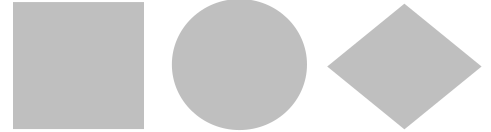
\includegraphics[scale=0.25]{./images/estruct_element.png}
	\end{center}
	\caption{Ejemplos de formas b\'asicas y compuestas de elementos estructurantes.}
\end{figure}

Sobre cada objeto de la imagen se pueden realizar operaciones l\'ogicas como \textbf{NOT}, \textbf{AND}, \textbf{OR} y \textbf{XOR}. Los objetos de una imagen al ser considerado un conjunto en la morfolog\'ia matem\'atica, las operaciones l\'ogicas sobre una imagen tiene una semejanza con las operaciones de conjuntos, las cuales son:

\begin{itemize}
	\item $A+B\rightarrow A\cup B$ (uni\'on)
	\item $A\cdot B \rightarrow A\cap B$ (intersecci\'on)
	\item $A\oplus B \rightarrow A\Delta B$ (diferencia sim\'etrica)
	\item $\bar{A} \rightarrow A^c$ (complemento)\\
\end{itemize}

Utilizando el lenguaje de conjuntos, se definen dos operaciones nombradas \textbf{dilataci\'on} y \textbf{erosi\'on}. \\\\
\textbf{\emph{Dilataci\'on: \\}}
Considerando A y B como conjuntos en $Z^2$. La dilataci\'on de A por B esta denotada por $A \oplus B$ y se define por la Ecuaci\'on 1.
\begin{equation}
	A \oplus B = \{z|(\bar{B})_z \cup A \neq 0 \}
\end{equation}
La dilataci\'on es el resultado de comprobar si el centro del elemento estructurante B coincide con uno o mas puntos del 
conjunto A. Cuando no ocurre, la imagen o conjunto A es un conjunto vac\'io.\\\\
\textbf{Erosi\'on: \\}
Consideramos A y B como conjuntos en $Z^2$. La erosi\'on de A por B denotada como $A \ominus B$ est\'a definida por la Ecuaci\'on 2.\\
\begin{equation}
	A \ominus B = \{z|(\bar{B})_z \subseteq A \}
\end{equation}

La transformaci\'on de erosi\'on es el resultado de comprobar si el elemento estructurante B est\'a totalmente incluido dentro del conjunto A. Cuando esto no ocurre, el resultado de la erosi\'on es el conjunto vac\'io.\\\\

Una vez definidas las transformaciones b\'asicas de la morfolog\'ia matem\'atica, se pueden utilizan combinando las operaciones, lo que da como resultado dos nuevas transformaciones llamadas \textbf{apertura} y \textbf{cerradura}\\\\

\textbf{Apertura: \\}
Se aplica la transformaci\'on de \textbf{erosi\'on}  seguida de una \textbf{dilataci\'on}, denotada por la Ecuaci\'on 3.\\
\begin{equation}
	A \circ B = \left( A \ominus B\right)\oplus B
\end{equation}

Al realizar esta transformaci\'on se obtiene distintos cambios en la imagen, los cuales son:
\begin{itemize}
	\item Suaviza los contornos de un objetos.
	\item Rompe istmos delgados
	\item Elimina salientes delgadas\\
\end{itemize}

\textbf{Cerradura: \\}
Se aplica la transformaci\'on de \textbf{dilataci\'on} seguida de una \textbf{erosi\'on} y se denota con la Ecuaci\'on 4.\\
\begin{equation}
	A \bullet B = (A \oplus B)\ominus B
\end{equation}
Como resultado de aplicar la transformaci\'on de \textbf{cerradura} son:
\begin{itemize}
	\item Suaviza
	\item Fusiona biscontinuidades
	\item Elimina agujeros pequen\~os
	\item Rellena huecos en el cotorno\\
\end{itemize}

\textbf{Extracci\'on de bordes}
Utilizando diferentes operaciones u orden de las mismas se pueden realizar distintos cambios en una imagen.\\
Para obtener los bordes de una imagen se puede realizar la operaci\'on denotada en la Figura 5.\\
\begin{equation}
	\beta (A) = A - \left(A \ominus B \right)
\end{equation}

 

\section{Metodolog\'ia}
Para cada transformaci\'on y la obtenci\'on de los bordes se han creado una funci\'on. Las funciones para la dilataci\'on y la erosi\'on tienen como argumentos la imagen de entrada y el elemento estructurante, a su vez, retornan un objeto de tipo \textbf{Mat}.\\
Se hizo de esta manera para poder utilizarlas en posteriores transformaciones como para la apertura y la cerradura, donde se utilizan ambas transformaciones pero en un orden diferente.\\\\
Para obtener la dilataci\'on de la imagen se debe comprobar que el centro del elemento estructurante coincide en su intensidad de gris con un pixel de la imagen. Si ambos valores coinciden se procede a dibujar el elemento estructurante sobre la imagen, tomando como centro del elemento estructurante el mismo pixel de la imagen.

\begin{figure}[h]
	\begin{center}
		\setlength{\unitlength}{0.00105in}
		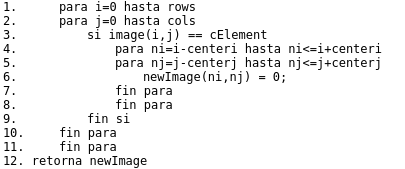
\includegraphics[scale=0.45]{./images/algoritmo1.png}
	\end{center}
	\caption{Pseudoc\'odigo para aplicar la transformaci\'on de dilataci\'on.}
\end{figure}

De acuerdo al pseudoc\'odigo de la Figura 2. con los dos primeros bucles anidados se recorre la imagen completa buscando el pixel del mismo tono de gris que el centro del elemento estructurante. Cuando dicho pixel es encontrado se ponen a 0 los p\'ixeles vecinos del pixel central, se toma el rango del vecindario de las mismas dimensiones que el elemento estructurante. Para ellos se usan otros dos bucles anidados que comienzan posicionandose en la esquina superior izquierda del vecindario, y con los mismo bucles se recorre cada elemento del vecindario cambiando su valor a 0. Al final se retorna la imagen resultante para aplicarla en otras transformaciones.\\

%1.		para i=0 hasta rows
%2.		para j=0 hasta cols
%3.			si image(i,j) == cElement
%4.				para ni=i-centeri hasta ni<=i+centeri 
%5.				para nj=j-centerj hasta nj<=j+centerj
%6.					newImage(ni,nj) = 0;
%7.				fin para
%8.				fin para
%9.			fin si
%10.		fin para
%11.		fin para
%12. retorna newImage

Para realizar la erosi\'on de una imagen nos podemos basar en el pseudoc\'odigo de la transformaci\'on de dilataci\'on, cambiando unicamente la manera en que cambiamos los valores a la vecindad del pixel central. Debido a que en la erosi\'on, el elemento estructurante debe ser un subconjunto de la figura a erosionar y, que de ser cumplirse esa condici\'on \'unicamente se debe cambiar o mantener el valor del pixel centra. Esto tendr\'a como resultado la disminusi\'on del tama\~no de las formas contenidas en la imagen.\\

Para obtener las transformaciones de \textbf{apertura} y \textbf{cerradura} se crearon dos funciones individuales, que tienen como argumentos la imagen de entrada y el elemento estructurante pero no retornan alg\'un valor u objeto ya que dentro de la misma funci\'on se muestran los resultados utilizando la funci\'on \textbf{plot} que solamente se creo para dicha acci\'on. Dentro se llaman las funciones de \textbf{erosi\'on} y \textbf{dilataci\'on}, dentro de sus propios argumentos se llamar las mismas funciones, ya sea dilataci\'on para la funci\'on de erosi\'on o viceversa. Al final se llama la funci\'on \textbf{plot} para mostrar los resultados.\\\\
Si queremos obtener los bordes de una imagen se creo su funci\'on individual. Dicha funci\'on como argumentos recibe la imagen de entrada y el elemento estructurante, como las dem\'as funciones, pero no retorna alg\'un valor u objeto, realizando la acci\'on de mostrar los resultados dentro de la funci\'on misma.

\section{Resultados}
Para realizar las pruebas se utilizaron como imagen base el resultado de la pr\'actica anterior, la binarizaci\'on de la imagen de unas monedas, y un elemento estructurante con forma de un cuadrado de 15x15 p\'ixeles, tal como se muestran en la Figura 3.

\begin{figure}[h]
	\begin{center}
		\setlength{\unitlength}{0.00105in}
		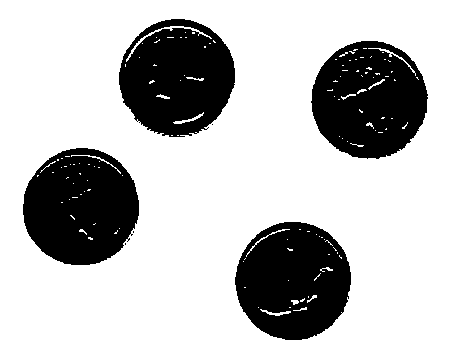
\includegraphics[scale=0.27]{./images/coins.png}
		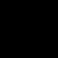
\includegraphics[scale=0.70]{./images/element.png}
	\end{center}
	\caption{La imagen de prueba es el resultado de la pr\'actica 5. El elemento estrucutrante no est\'a a escala, s\'olo es para mostrar su forma.}
\end{figure}

Como resultado de la transformaci\'on de dilataci\'on el resultado esperado ser\'a eliminar los puntos blancos dentro de los objetos negros(monedas), siendo el resultado el mostrado en la Figura 4. Podemos observar que adem\'as de cubrir los huecos o puntos blancos dentro de las monedas, tambi\'en se aumento del taman\~o de las mismas debido a las dimensiones y forma del elemento estructurante.

\begin{figure}[h]
	\begin{center}
		\setlength{\unitlength}{0.00105in}
		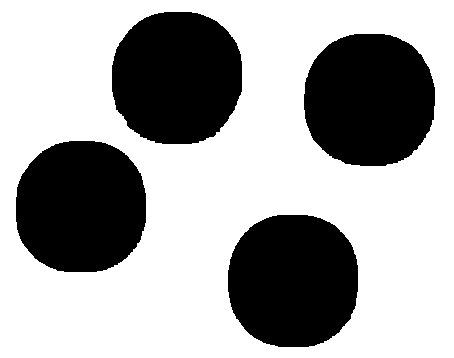
\includegraphics[scale=0.30]{./images/coins_out.png}
	\end{center}
	\caption{Resultado al aplicar la dilataci\'on a la imagen de las monedas.}
\end{figure}

El resultado de aplicar la erosi\'on sobre la imagen de las monedas se puede ver en la Figura 5.
\begin{figure}[h]
	\begin{center}
		\setlength{\unitlength}{0.00105in}
		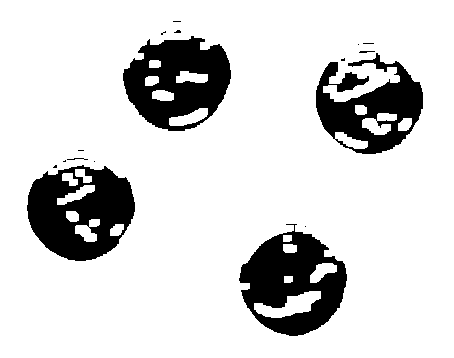
\includegraphics[scale=0.30]{./images/erosion_out.png}
	\end{center}
	\caption{Resultado al aplicar la erosi\'on a la imagen de las monedas.}
\end{figure}

Cuando aplicamos primero la erosi\'on y enseguida la dilataci\'on a la imagen de las monedas que se muestra en la Figura 6.
\begin{figure}[h]
	\begin{center}
		\setlength{\unitlength}{0.00105in}
		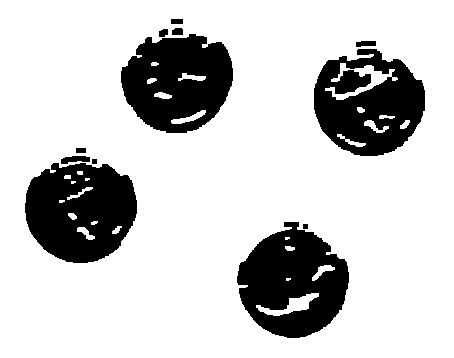
\includegraphics[scale=0.30]{./images/apertura_out.png}
	\end{center}
	\caption{Resultado de aplicar la operaci\'on de apertura a la imagen de las monedas.}
\end{figure}
De la misma manera, si aplicamos primero la dilataci\'on y enseguida la erosi\'on el resultado es el que se ve en la Figura 7.
\begin{figure}[h]
	\begin{center}
		\setlength{\unitlength}{0.00105in}
		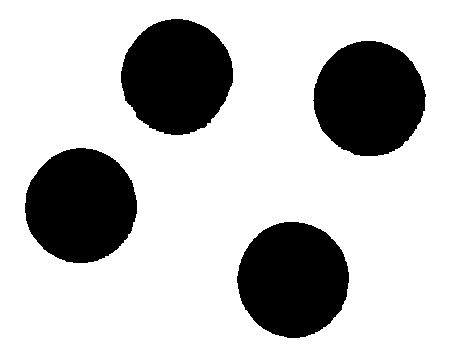
\includegraphics[scale=0.26]{./images/cerradura_out.png}
	\end{center}
	\caption{Resultado de aplicar la operaci\'on de cerradura a la imagen de las monedas.}
\end{figure}

\newpage
Cuando hacemos la diferencia entre la imagen original menos la erosi\'on de la imagen obtenemos los bordes, en este caso, los bordes de la imagen de las monedas se muestra en la Figura 8. Para esta transformaci\'on es necesario cambiar el elemento estructurante a un cuadrado de 3x3 pixeles.

\begin{figure}[h]
	\begin{center}
		\setlength{\unitlength}{0.00105in}
		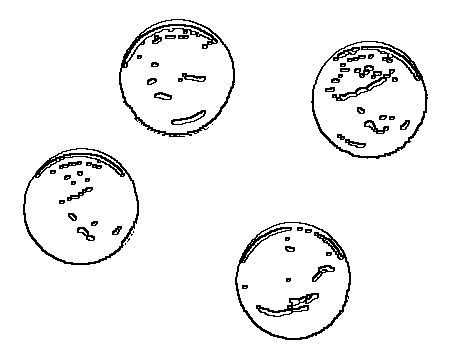
\includegraphics[scale=0.30]{./images/bordes_out.png}
	\end{center}
	\caption{Resultado de aplicar la operaci\'on para obtener los bordes de la imagen de las monedas.}
\end{figure}

\section{Conclusiones}
Las transformaciones de dilataci\'on y erosi\'on tienen muchas aplicaciones, tanto individuales como en conjunto. Un punto sumamente importante es que el resultado de aplicar las trasnformaciones no s\'olo depende de las mismas operaciones, los resultados son muy dependientes de la forma del elemento estructurante, se debe elegir una forma ``ideal'' para cada imagen ya que no siempre pueden darse los resultados deseados con una forma en com\'un.


%\begin{thebibliography}{1}
%    \bibitem{IEEEhowto:kopka}
%    H.~Kopka and P.~W. Daly, \emph{A Guide to \LaTeX}, 3rd~ed.\hskip 1em plus
%      0.5em minus 0.4em\relax Harlow, England: Addison-Wesley, 1999.
%\end{thebibliography}

%\begin{IEEEbiography}[{\includegraphics[width=1in,height=1.25in,clip,keepaspe%ctratio]{picture}}]{John Doe}
%\blindtext
%\end{IEEEbiography}

\end{document}